\documentclass[15pt]{article}
\usepackage{fullpage}
\usepackage{graphicx}
%\usepackage{multicol}
\usepackage{tabularx}
%\setlength{\columnsep}{1cm}

\begin{document}
\begin{center}
	\huge{\textbf{Akshay Vijay Bhosale}} \\
\end{center}
\noindent \hrulefill
\begin{flushleft}
	\large{
		Flat No.301, \hfill
		Contact: 9740402335  \\
		Aditya Heights, \hfill 	email-id: akshaybhosale526@gmail.com \\
		Vijayanagar 3rd Cross, \\
		Hindalga Road, \\
		Belagavi-590118.}
\end{flushleft}
\begin{center}
	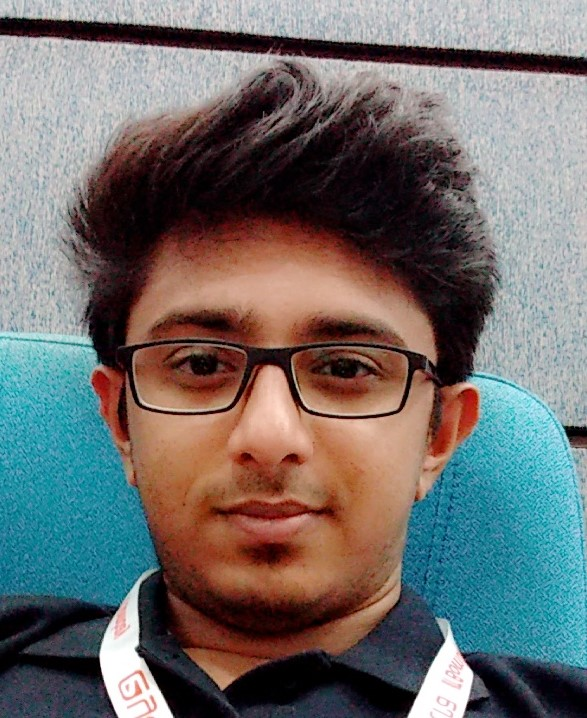
\includegraphics[scale=0.15]{pic.PNG}
\end{center}
\vspace{1mm}
\begin{flushleft}
	{\textbf{Objective }} \\
	\vspace{0.5mm}
	\noindent \hrulefill
	\vspace{0.5mm} \\
	An electronics and communication third year undergraduate student seeking opportunities in the field of embedded systems, robotics and computer vision. \\
\end{flushleft}
\vspace{1mm}
\begin{flushleft}
	{\textbf{Education }} \\
	\vspace{0.5mm}
	\noindent \hrulefill 
	\vspace{0.5mm} \\
	\begin{tabular}{|p{3cm}|p{3cm}|p{3cm}|c|p{3cm}|}
		\hline
		Degree & College/School & University/Board & Passing Year & Percentage/CGPA \\
		\hline 
		B.E Electronics and Communication & K.L.S Gogte Institute of Technology, Belgaum & Autonomous Institute under Visvesvaraya Technological University & 2019 & 9.20(Sem 1 to Sem 5) \\
		\hline
		XII (Senior Secondary), Science & R.L.S college, Belgaum & Department of Pre-University education, Karnataka & 2015 & 89.5$\%$ \\
		\hline
		X (Secondary) & B.M.E.M.H.S, Dharwad & Karnataka Secondary Education Examination Board & 2013 & 95.04$\%$ \\
		\hline
	\end{tabular}
\end{flushleft}
\vspace{1mm}
\begin{flushleft}
	{\textbf{Projects}} \\
	\vspace{0.5mm}
	\noindent \hrulefill 
	\vspace{0.5mm} \\
	\begin{enumerate}
		\item Harvestor Bot for E-Yantra Robotics Competition 2017-18. \begin{enumerate}
			\item Autonomous robot developed for harvesting of fruits.
			\item Uses Image Processing techniques for fruit identifaction.
		\end{enumerate} 
		\item Automatic Helmet Detection using Neural Networks. [Ongoing]
		\begin{enumerate}
			\item Trained neural networks classify bikes and other vehicles.
			\item Another neural network is used to differentiate between a biker with and without helmet.
		\end{enumerate}
		\item Advanced Water Level Controller Using Arduino.
		\begin{enumerate}
			\item Automatically detects the water level, indicates on an LCD and controls the motor.
		\end{enumerate}
		\item Androbot.
		\begin{enumerate}
			\item Bluetooth controlled robot.
			\item Additional feature:- Obstacle Detection.
		\end{enumerate}
		\item Sixth sense robot.
		\begin{enumerate}
			\item Uses colour detection to traverse.
			\item Serial communication between PC and robot.
		\end{enumerate}
	\end{enumerate}
\end{flushleft}
\vspace{1mm}
\begin{flushleft}
	{\textbf{Trainings and Internships}} \\
	\vspace{0.5mm}
	\noindent \hrulefill 
	\vspace{0.5mm} \\
	\begin{itemize}
		\item Course on Machine Learning [Ongoing]
		\item Introduction to digital image and video processing.
		\item Participated in a workshop on Sixth Sense Robotics conducted at IIT Bombay during TechFest 2016-17.
		\item Participated in Androbot workshop conducted by TechKriti, the annual Technical and Entrepreneurial Festival of IIT Kanpur, 2016.
	\end{itemize}
\end{flushleft}
\vspace{1mm}
\begin{flushleft}
	{\textbf{Research Publications}} \\
	\vspace{0.5mm}
	\noindent \hrulefill 
	\vspace{0.5mm} \\
	\begin{enumerate}
		\item None
	\end{enumerate}
\end{flushleft}
\vspace{1mm}
\begin{flushleft}
	{\textbf{Papers Presented}} \\
	\vspace{0.5mm}
	\noindent \hrulefill 
	\vspace{0.5mm} \\
	\begin{enumerate}
		\item Image Recovery Using Neural Networks.
	\end{enumerate}
\end{flushleft}
\vspace{1mm}
\begin{flushleft}
	{\textbf{Technical Skills}} \\
	\vspace{0.5mm}
	\noindent \hrulefill 
	\vspace{0.5mm} \\
	\begin{itemize}
		\item \textbf{Programming Languages :-} C, Matlab, Python, Embedded C, ARM Assembly.
		\item \textbf{Hardware Knowledge :-} ATmega microcontrollers, Arduino, Raspberry Pi, LPC2148.
		\item \textbf{Software Knowledge :-}
		Familiar with OpenCV and Numpy libraries and tools such as Cadence Virtuoso, Multisim, Xilinx ISE, Keil uVision 4.
	\end{itemize}
\end{flushleft}
\vspace{1mm}
\begin{flushleft}
	{\textbf{Soft Skills}} \\
	\vspace{0.5mm}
	\noindent \hrulefill 
	\vspace{0.5mm} \\
	\begin{enumerate}
		\item Flexibility, Dedication, Teamwork, Communication, Responsibility.
		\item Cleared Cambridge English: Business Preliminary (BEC Preliminary) with B2 certification level.
	\end{enumerate}
\end{flushleft}
\vspace{1mm}
\begin{flushleft}
	{\textbf{Extra Curricular activities}} \\
	\vspace{0.5mm}
	\noindent \hrulefill 
	\vspace{0.5mm} \\
	\begin{itemize}
		\item Part of the plantation drive conducted by Naviours group in the city of belagavi.
		\item Co-ordinated and organized various events during Aura, the cultural fest of K.L.S GIT Belagavi.
	\end{itemize}
\end{flushleft}
\vspace{1mm}
\begin{flushleft}
	{\textbf{Co-Curricular activities}} \\
	\vspace{0.5mm}
	\noindent \hrulefill 
	\vspace{0.5mm} \\
	\begin{enumerate}
		\item Secured \textbf{1st Prize} in E-Yantra Robotics Competition 2017-18 in the theme Harvestor Bot.
		\item Secured \textbf{1st Place} in Flipped Logic, an event under Panchajanya'16, a Tech-Fest held at K.L.S GIT, belagavi.
		\item Secured \textbf{1st Place} in Lazer Mazer, an event under Panchajanya'16, a Tech-Fest held at K.L.S GIT, belagavi.
	\end{enumerate}
\end{flushleft}
\vspace{1mm}
\begin{flushleft}
	{\textbf{Personal Details}} \\
	\vspace{0.5mm}
	\noindent \hrulefill 
	\vspace{0.5mm} \\
	\begin{itemize}
		\item \textbf{Father's Name :-} Vijay P Bhosale
		\item \textbf{Mother's Name :-} Bharati V Bhosale
		\item \textbf{Sex :-} Male
		\item \textbf{Date of Birth :-} 26 May 1997
		\item \textbf{Nationality :-} Indian
		\item \textbf{Marital Status :-} Single
	\end{itemize}
\end{flushleft}
\vspace{1mm}
\begin{flushleft}
	{\textbf{References}} \\
	\vspace{0.5mm}
	\noindent \hrulefill 
	\vspace{0.5mm} \\
	\begin{enumerate}
		\item Dr. Prashant Patavardhan, Head of Department, Electronics and Communication Engineering, K.L.S GIT belagavi$|$pppatavardhan@git.edu$|$944891840.
		\item Prof. Supriya S Shanbhag, Assistant Professor, Electronics and Communication Engineering, K.L.S GIT belagavi$|$ssshanbhag@git.edu$|$9845306767.
	\end{enumerate}
\end{flushleft}
\end{document}